\chapter{Evaluation}
\label{Evaluation}

In order to evaluate the quality of the \aicat\ framework, several
aspects of the framework have been tested.  The three main areas
tested are quality of categorization, efficiency, and ease of use.
For testing the quality of categorization and efficiency, performance
is measured on categorization tasks using several different data sets.

Section \ref{Corpora} describes the data sets used during testing.
Section \ref{Quality} presents various measurements of how accurately
the framework performs on these data sets, and Section
\ref{Efficiency} discusses the computational efficiency of the
framework.  Section \ref{Applications} discusses the ease of use of
the framework in different contexts.


\section{Corpora}
\label{Corpora}

During development and testing, several data sets, or ``corpora,''
were used for framework testing and application building.  Since the
framework will behave differently on different data sets, it is
important to understand the characteristics of each corpus.  For
instance, different feature selection and categorization algorithms
may scale differently in relation to the size of the training corpus,
both in terms of efficiency and accuracy.\cite{chakrabarti:98} Also,
the specifics of the categorization problem in each corpus may be more
amenable to one categorization technique or another.

The main corpora used for evaluation are listed in this section.  Each
corpus consists of a set of documents $\docs$, a set of categories $\cats$ that
documents may be assigned to, and a domain-expert-made choice of
category assignments for each document.  These category assignments
are considered to be completely correct, and they form a standard
against which the TC system's categorization on the test documents can
be measured.  For each corpus, the set $\docs$ is divided into a
training set $\train$ and a test set $\test$.

Unless otherwise noted below, a list of common English words from
\cite{salton:89} was used as a ``stoplist,'' or a set of terms to
completely ignore when processing documents.  This is a common technique from
Information Retrieval,\cite{XXX-manning} as it is assumed that these words
possess little or no information about the target categories, and that
they will only slow processing and add noise to the data.


\subsection{ApteMod}


The ApteMod version of the Reuters-21578 corpus has become a
standard benchmark corpus in evaluating Text Categorization
systems.\cite{yang:99} It is a collection of 10,788 documents from the
Reuters financial newswire service, partitioned into a training set with 7769
documents and a test set with 3019 documents.  The total size of the
corpus is about 43 MB.  It is available for download from
\url{http://kdd.ics.uci.edu/databases/reuters21578/reuters21578.html}.

The distribution of categories in the ApteMod corpus is highly skewed,
with 36.7\% of the documents in the most common category, and only
0.0185\% (2 documents) in each of the five least common categories.
In fact, the original data source is even more skewed---in creating
the corpus, any categories that did not contain at least one document
in the training set and one document in the test set were removed from
the corpus.\cite{yang:99}

In the ApteMod corpus, each document belongs to one or more
categories.  There are 90 categories in the corpus.  The average
number of categories per document is 1.235, and the average number of
documents per category is about 148, or 1.37\% of the corpus.

Figure \ref{Corpora-catdist} shows the category distribution for all
four corpora discussed in this section.  The categories are plotted on
the horizontal axis, and the number of documents per category are
plotted on the vertical axis using a logarithmic scale.

\begin{figure}
\begin{center}
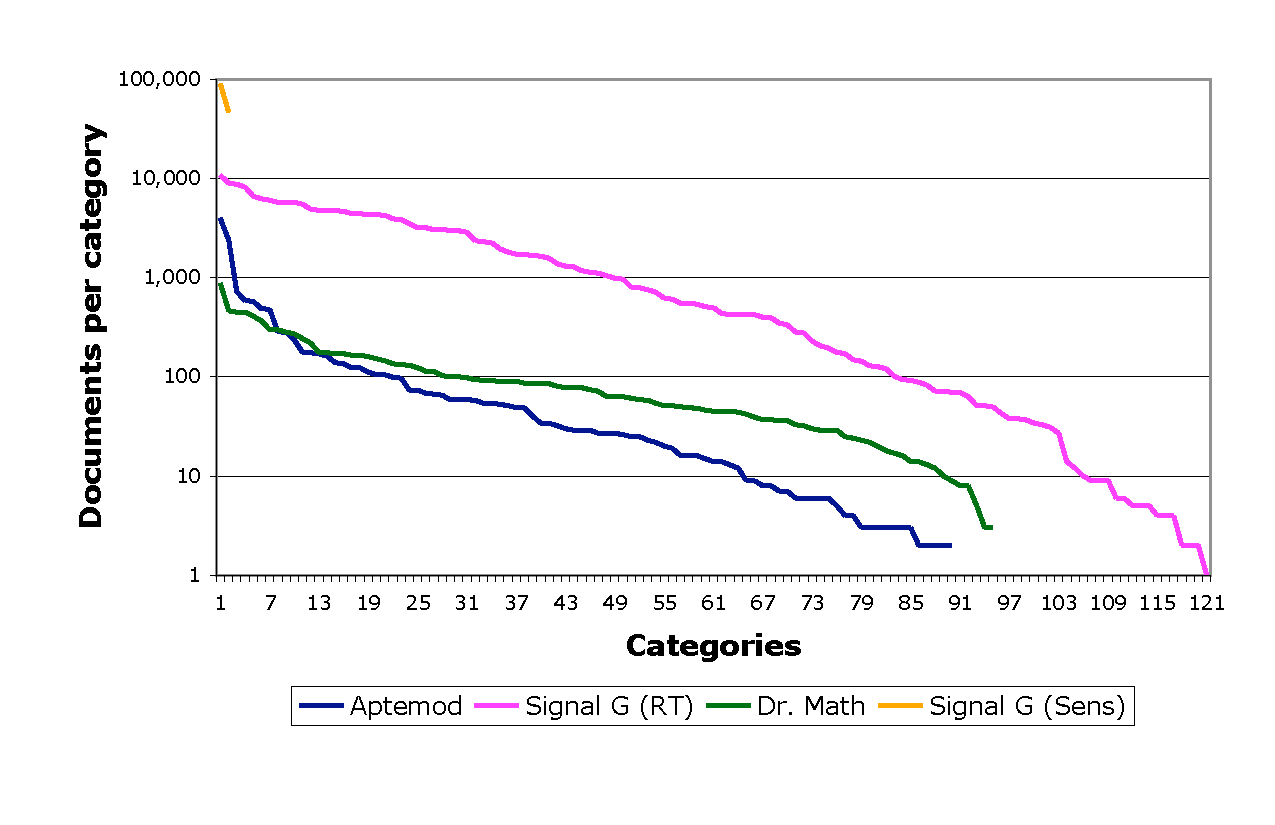
\includegraphics[width=\linewidth]{figures/Corpora-catdist.pdf}
\caption{Category distribution for the four test corpora}
\label{Corpora-catdist}
\end{center}
\end{figure}


\subsection{Dr. Math}

The Dr. Math corpus is a collection of 6,630 English-language messages
sent to the ``Ask Dr. Math'' question-and-answer service for
students.\cite{drmath} Each message has been manually assigned by a
domain expert to one or more categories,
with category names indicating both math topic and grade level,
e.g. ``High School Geometry.''  There are 95 categories in the
category set.  The ontology is generally not
separable into two separate category sets for independent topic and
level categorizations, in part because many topic and level
combinations like ``Elementary School Calculus'' don't exist in the
category scheme.

The 26 MB corpus is divided into a training set with 5,304 documents
and a test set with 1,326 documents.  As with the ApteMod corpus, the
category distribution is skewed, with 13.2\% of the documents in the
most common category and only 0.0452\% (3 documents) in the least
common category.  The average number of categories per document is
1.534, and the average number of documents per category is about 107,
or 1.61\% of the corpus.

The corpus is not available for direct download, but interested
parties may contact the author for details.


\subsection{Signal G (Sensitivity)}

The Signal G corpus consists of 136,630 financial announcement
documents from the Australian Stock Exchange (ASX)\cite{asx:02} issued
between January 4 and December 29, 2000.  Each documents has been
manually categorized by the ASX according to whether it indicates ``market
sensitivity'' or not.  Market sensitivity is a subjective label indicating
whether the given document has potential to affect the issuing
company's share value, trading volume, or other properties on the
exchange.  Every document is a member of either the ``sensitive'' or
``insensitive'' category---this can be viewed as two categories that
partition the corpus, or as a single category that some documents
belong to and others don't.  This discussion assumes the former.

The documents are divided into a training set of 95,525 documents and a
test set of 41,105 documents.  The total size of the corpus is about
342 MB.  Of the 136,630 corpus documents, about 34.0\% are marked as
market sensitive, and the rest are marked as insensitive.

\subsection{Signal G (Report Type)}

The same documents in the previous corpus can also be tagged with a
``report type'' category.  This category indicates the type of
business announcement contained in the document, and may take values
such as ``Notice of Annual General Meeting'' or ``Dividend Books
Closing.''  There are 121 categories in the corpus, with 7.91\%
(10,815 documents) belonging to the most common category, and ten
categories that contain five documents or fewer.  Thus the corpus
exhibits a high skew with respect to this category scheme, similar to
the ApteMod and Dr. Math corpora.

For this corpus with the Report Type labels, the same division between
training and test documents was used as with the Sensitivity labels.



\section{Quality of Categorization}
\label{Quality}

In order to evaluate the quality of the results generated by automatic
categorization systems, researchers usually evaluate the results of
the system on a controlled set of test documents which have manually
been assigned category labels by a human expert.
\cite[pp. 9 \& 37]{sebastiani:02} This is the approach used here,
using the four corpora described in Section \ref{Corpora} as the test
sets.

It should be emphasized that this thesis does not claim to produce any
new results in the area of developing Text Categorization algorithms.
Descriptions of existing algorithms from the TC literature have formed
the basis for developing the \aicat\ framework.  The results presented
here should be considered successful if they align with results
already published in the literature---superior results should not be
expected.

\subsection{Performance Measures}
\label{measures}

Several statistical measures have become standard in the area of
evaluating Text Categorization systems.\cite[p. 33]{sebastiani:02}
Some of the most prevalant are based on the notions of
\emph{precision} and \emph{recall} from the field of Information
Retrieval.\cite{rijsbergen:79} Precision, often denoted by the symbol
$\pi$, measures the probability that a document assigned by the TC
system to a given category actually belongs to that category.
Conversely, recall, denoted by $\rho$, measures the probability that a
document actually belonging to a certain category will be assigned
during testing to that category.\cite[p. 33]{sebastiani:02}

The probabilities mentioned above can be estimated during testing by
comparing how often the TC system's category choices match the correct
categories.  A valuable tool for this analysis is the ``contingency
table,'' which summarizes the results of the experiment for a given
category.  Table \ref{onecat-contingency} shows a contingency table
for the category $c_i$, i.e. any arbitrary category in the
categorization scheme of the corpus.  Here, $A_i$, etc. represent the
number of documents that fall into the given situation, i.e. $A_i$ is
the number of test documents assigned to category $c_i$ by both the
expert and the TC system.

This allows us to estimate $\pi$ and $\rho$, whose true values are
$P(Expert=Y | System=Y)$ and $P(System=Y | Expert=Y)$, respectively,
in terms of the entries in the contingency table.  Since the number of
documents assigned to category $c_i$ by the TC system is $A_i+B_i$,
and the number assigned by the expert is $A_i+C_i$, our estimates for
$\pi$ and $\rho$ are $\frac{A_i}{A_i + B_i}$ and $\frac{A_i}{A_i +
C_i}$, respectively.



\begin{table}
\begin{center}
\begin{tabular}{|c|c|c|c|}
\cline{3-4}
\multicolumn{2}{c|}{} & \multicolumn{2}{c|}{\textbf{Expert choice}} \\
\cline{3-4}
\multicolumn{2}{c|}{} & Yes & No \\
\hline
\textbf{System} & Yes & $A_i$ & $B_i$ \\
\cline{2-4}
\textbf{choice} & No  & $C_i$ & $D_i$ \\
\hline
\end{tabular}
\end{center}
\caption{Contingency table for category $c_i$}
\label{onecat-contingency}
\end{table}


$\pi$ and $\rho$ give valuable information about the performance of a
TC system, but neither provides an isolated rating of the system's
quality.  The reason is that either measure can usually be improved in
a system to the detriment of the other.\cite[p. 35]{sebastiani:02} For
instance, the \emph{trivial acceptor} categorizer, which assigns every
document to every category, will have a perfect $\rho$ score of 1, but
its precision will be unacceptably low on any nontrivial task.

Therefore, a measure that combines $\pi$ and $\rho$ is desirable as an
overall measure of the quality of the TC system.  One such measure is
the $F_\beta$ measure, first introduced to the Information Retrieval
literature by van Rijsbergen \cite[ch. 7]{rijsbergen:79}.  It is
defined by the equation $F_\beta = \frac{(\beta^2 + 1)\pi\rho}{\beta^2
\pi + \rho}$, where $0 \leq \beta \leq \infty$.  The $\beta$ parameter
provides a continuous way to balance between the importance of $\pi$
and $\rho$, with values closer to 0 emphasizing $\pi$, values closer
to $\infty$ emphasizing $\rho$, and a value of 1 balancing the two
measures equally.  Without specific knowledge of an application's
requirements (for instance, whether false positives for a certain
category are more problematic than false negatives), one may presume
that $\pi$ and $\rho$ are equally important, and therefore the
literature often uses $F_1$ as a measure of the quality of a TC system
on a particular category.

${F_1}_i$ may be derived in terms of the entries of the per-category
contingency table as follows:

\begin{equation*}
\begin{split}
{F_1}_i 
 & = \frac{ 2 \pi_i \rho_i}{\pi_i + \rho_i} \\[6pt]
 & = \frac{ \frac{2 {A_i}^2}{(A_i+B_i)(A_i+C_i)} } { \frac{A_i}{A_i+B_i} + \frac{A_i}{A_i+C_i} } \\[6pt]
 & = \frac{ 2 {A_i}^2 }                            { A_i(A_i+C_i) + A_i(A_i+B_i) } \\[6pt]
 & = \frac{ 2 A_i }                                { 2 A_i + B_i + C_i } \\[6pt]
\end{split}
\end{equation*}

Two other measures of categorization quality, \emph{error} and
\emph{accuracy}, are also sometimes encountered in the TC literature.
These are simple measures which can also be defined in terms of the
contingency table in Table \ref{onecat-contingency}: $error =
\frac{B_i+C_i}{A_i+B_i+C_i+D_i)}$, and $accuracy =
\frac{A_i+D_i}{A_i+B_i+C_i+D_i)}$.  In other words, error is the
proportion of the system's decisions that matched the expert's
choices, and accuracy is the proportion that did not.  As summarized
in \cite[p. 34]{sebastiani:02}, these are not always useful measures
of categorization quality, because the \emph{trivial rejector} (a
system that never assigns any documents to any category) will often
have a lower error and higher accuracy than most nontrivial
categorizers.  Nonetheless, error will be measured for the evaluation
tasks here, because it may give insight into the character of the
system's performance.


\subsection{Combining Measures Across Categories}
\label{combining-measures}

Section \ref{measures} introduced several performance measures that
may be defined to evaluate a categorizer on a single category.  In
order to evaluate the categorizer's overall performance on the entire
set of test documents, it is desirable to combine the per-category
scores $\pi_i$, $\rho_i$, and ${F_1}_i$ into overall scores for the
entire category set.

Two methods for doing this are standard in the literature.  The first
is called \emph{micro-averaging}, and sums the terms in the
contingency table for all categories simultaneously rather than in
per-category tables.  In other words, the micro-averaged $\pi$,
$\rho$, and $F_1$, notated $\pi^\mu$, $\rho^\mu$, and $F^\mu_1$, are
defined in terms of the per-category contingency tables by the
following equations.

\begin{equation*}
 \pi^\mu = \frac{\sum_{i=1}^{|C|}{A_i}} {\sum_{i=1}^{|C|}{A_i+B_i}} \qquad
\rho^\mu = \frac{\sum_{i=1}^{|C|}{A_i}} {\sum_{i=1}^{|C|}{A_i+C_i}} \qquad
 F^\mu_1 = \frac{\sum_{i=1}^{|C|}{2 A_i}} {\sum_{i=1}^{|C|}{2 A_i+B_i+C_i}} \qquad
\end{equation*}

Micro-averaging gives equal weight to each categorization decision
made by the system, or equivalently, to each document in the corpus,
regardless of how many categories it belongs to.

An alternative to micro-averaging is \emph{macro-averaging}, in which
the per-category scores $\pi_i$, $\rho_i$, and ${F_1}_i$ are simply
averaged to find the macro-averaged $\pi$, $\rho$, and $F_1$, notated
$\pi^M$, $\rho^M$, and $F^M_1$.  The following equations describe this
procedure.

\begin{equation*}
 \pi^M = \frac{\sum_{i=1}^{|C|}{\pi_i}}   {|C|} \qquad
\rho^M = \frac{\sum_{i=1}^{|C|}{\rho_i}}  {|C|} \qquad
 F^M_1 = \frac{\sum_{i=1}^{|C|}{{F_1}_i}} {|C|} \qquad
\end{equation*}

Macro-averaging gives equal weight to each category in the corpus,
regardless of how many documents it contains.  Thus it provides a
good counterpart to micro-averaging; macro-averaging will place more
emphasis on rare categories than micro-averaging, so reporting both
scores is typically useful to evaluate the system as a whole.

Note that the error and accuracy measures are unaffected by micro-
vs. macro-averaging, as shown in the following derivation.  This uses
the observation that $A_i+B_i+C_i+D_i = |\test|$, a consequence of the
fact that exactly one of the terms on the left side will be
incremented with each decision about whether a document from the test
set belongs to $c_i$ or not.

\begin{equation*}
\begin{split}
error^M
 & = \frac{\sum_{i=1}^{|\cats|}{error_i}}  {|\cats|} \\[6pt]
 & = \frac{\sum_{i=1}^{|\cats|}{ \frac{B_i+C_i}{A_i+B_i+C_i+D_i} }} { \sum_{i=1}^{|\cats|}{1} } \\[6pt]
 & = \frac{\sum_{i=1}^{|\cats|}{ \frac{B_i+C_i}{|\test|} }}         { \sum_{i=1}^{|\cats|}{1} } \\[6pt]
 & = \frac{\sum_{i=1}^{|\cats|}{B_i+C_i}}                           { \sum_{i=1}^{|\cats|}{|\test|} } \\[6pt]
 & = \frac{\sum_{i=1}^{|\cats|}{B_i+C_i}}                           { \sum_{i=1}^{|\cats|}{A_i+B_i+C_i+D_i} } \\[6pt]
 & = error^\mu
\end{split}
\end{equation*}


\subsection{Results}

Using the measures defined in Sections \ref{measures} and
\ref{combining-measures}, categorization experiments were performed on
each of the four corpora described in Section \ref{Corpora}.  Several
experimental parameters (e.g. category membership thresholds) can be
set for each experiment; for the ApteMod corpus these were set to
match the parameters used in \cite{yang:99}, where known.  For the
other corpora they were optimized to provide the
best performance on the test set---in this sense, the test set might
be thought of more correctly as a validation set, because in a strict
testing environment the performance on the test set should not
influence training parameters.  This methodology was adopted because
it more closely matches the procedure that would be used when building
an application, in which the true test set may consist of documents
not yet posessed by the developer, i.e. the set of target documents
in the application domain.

Where a baseline score is given in the results, this refers to a
simple probabilistic categorizer that assigns categories to each
document, weighting the probability of assignment by the frequency of
each category in the training set.  For instance, if a certain
category was present in 40\% of the training documents, any document
in the test set would have a probability of 0.4 of being assigned to
that category by the baseline categorizer.  

\subsubsection{ApteMod}

Table \ref{aptemod-results} summarizes the results of three different
machine learning methods in \aicat\ as compared with the baseline
categorizer described above.  Table \ref{aptemod-yang} gives similar
scores from a well-known comparitive study of common categorization
algorithms.\cite{yang:99} Where possible, the present study has
attempted to duplicate the findings in \cite{yang:99}, though in some
cases there is not enough information to duplicate the findings
exactly, and in some cases the \aicat\ framework lacks certain
features mentioned in \cite{yang:99}.  These differences will be
discussed below.

\begin{table}
\begin{center}
\begin{tabular}{|r c c c c c c c|}
\hline
%              maR       maP       maF1      miR          miP         miF1
method    & $\rho^M$ & $\pi^M$ & $F_1^M$ & $\rho^\mu$ & $\pi^\mu$ & $F_1^\mu$ &   error \\
\hline
NB        &   .3659  &  .4969  &  .3959  &  .7238     &  .8514    &  .7824    &  .00555 \\
SVM       &   .0868  &  .3727  &  .1239  &  .5254     &  .9106    &  .6663    &  .00725 \\
kNN       &   .2655  &  .3856  &  .2903  &  .7650     &  .7975    &  .7809    &  .00591 \\
Baseline  &   .0135  &  .0142  &  .0137  &  .1645     &  .1664    &  .1654    &  .02287 \\
\hline
\end{tabular}
\end{center}
\caption{Results of \aicat\ on ApteMod corpus}
\label{aptemod-results}
\end{table}

\begin{table}
\begin{center}
\begin{tabular}{|r c c c c c c c|}
\hline
method & $\rho^M$ & $\pi^M$ & $F_1^M$ & $\rho^\mu$ & $\pi^\mu$ & $F_1^\mu$ & error \\
\hline
NB  & ? & ? & .3886 & .7688 & .8245 & .7956 & .00544 \\
SVM & ? & ? & .5251 & .8120 & .9137 & .8599 & .00365 \\
kNN & ? & ? & .5242 & .8339 & .8807 & .8567 & .00385 \\
\hline
\end{tabular}
\end{center}
\caption{Results from \cite{yang:99} on ApteMod corpus}
\label{aptemod-yang}
\end{table}

In the case of the \naive\ Bayes categorizer (NB), the results match
\cite{yang:99} closely, with a slightly greater $F_1^M$ and a slightly
smaller $F_1^\mu$. (XXX - not sure whether I can say that the
differences are statistically insignificant or not.  Need to
understand Yang's stats tests better?)  To match the experimental
settings in \cite{yang:99}, the size of the feature-set was set to
2000.

For the Support Vector Machine categorizer (SVM), the performance is
significantly worse than the findings in \cite{yang:99}.  The reasons
for this are not clear---\aicat\ currently uses an SVM implementation
based on the \texttt{libsvm} C library \cite{libsvm}, whereas
\cite{yang:99} used $SVM^{light}$ as its
implementation\cite{joachims:99a}, and there may be major differences
in the behavior of these two libraries.  Since the macro-averaged scores are
particularly bad, it may be inferred that \cite{libsvm} is not
performing well on rare categories.  In both studies, a linear SVM
kernel was used, and 10,000 features were considered when building the
categorization model.

One possible reason for the poor performance of the SVM categorizer is
that for both micro- and macro-averaged scores, $\pi$ is much larger
than $\rho$, indicating that this situation could be balanced by
choosing more appropriate category membership thresholds.  However,
\texttt{libsvm} doesn't seem to allow tuning of these thresholds, so a
remedy for this situation isn't clear.

For the k-Nearest-Neighbor categorizer (kNN), $F_1^\mu$ results are comparable
with NB, but no scores are as good as the kNN results in \cite{yang:99}.
The major difference between the two implementations is that the
implementation in \cite{yang:99} finds per-category membership
thresholds by optimizing performance on a validation set, while the
implementation in \aicat\ uses a single membership threshold for all
categories, settable by the user.  In this experiment the threshold
was set to 0.1, a value which is not meaningful in itself, but which
seemed to give the best performance.  Note, that the macro-averaged
precision is higher than recall, but the micro-averaged recall is
higher than precision, indicating that it is not possible to
simultaneously find the optimal threshold for both rare and common
categories.  Thus using individual thresholds for each category should
increase $F_1$ scores if optimized properly.  The $k$ parameter
in this experiment
(indicating the number of similar documents to consider when
categorizing) was set to 45, and the number of features considered was
set to 2415, both to match the values used in \cite{yang:99}.

The kNN implementation in \aicat\ is fairly new, and is an adaptation
of work by another researcher.  The ability to optimize per-category
thresholds is considered a useful future addition to the framework,
and will be added soon.

For all three categorizers, the \param{tfidf\_weighting} parameter was set to
\texttt{xfx}, indicating that words are weighted by the logarithm of
their inverse document frequency.  This is the same setting used in
\cite{yang:99}.  One other possible difference between \cite{yang:99}
and the current experiment is that \cite{yang:99} used either a
$\chi^2$ or \emph{information gain} criterion (it is not clear which
criterion was used with which categorizer) for feature selection,
while \emph{document frequency} was used here.  This should not be a
major factor in the results, as document frequency has been shown to
produce results competitive with other feature selection methods on
this corpus. \cite{yang:97}



\subsubsection{Dr. Math}

Table \ref{drmath-results} shows the categorization performance of
\aicat\ on the Dr. Math corpus.  Note that the baseline micro-averaged
scores are much lower than on the ApteMod corpus (Table
\ref{aptemod-results}), indicating that this may be a more difficult
categorization task simply because the category distribution is
flatter than in ApteMod (Figure \ref{Corpora-catdist}).


\begin{table}
\begin{center}
\begin{tabular}{|r c c c c c c c|}
\hline
%              maR       maP       maF1      miR          miP         miF1
method    & $\rho^M$ & $\pi^M$ & $F_1^M$ & $\rho^\mu$ & $\pi^\mu$ & $F_1^\mu$ &   error \\
\hline
NB        &   .2338  &  .2677  &  .2358  &  .3766     &  .3542    &  .3651    &  .0215  \\
SVM       &   .3333  &  .1562  &  .1946  &  .4211     &  .2273    &  .2952    &  .0330  \\
kNN       &   .2372  &  .2824  &  .2154  &  .3607     &  .3572    &  .3590    &  .0212  \\
Baseline  &   .0156  &  .0176  &  .0161  &  .0406     &  .0421    &  .0413    &  .0310  \\
\hline
\end{tabular}
\end{center}
\caption{Results of \aicat\ on Dr. Math corpus}
\label{drmath-results}
\end{table}

Because no other TC study has been done on the Dr. Math corpus, not
much can be said about the comparitive results of the \aicat\
framework.  However, the noteworthy points will be discussed below.

Using the \naive\ Bayes categorizer, the $F_1$ scores are about 0.24
when macro-averaged and 0.37 when micro-averaged.  This is not as
dramatic a difference as seen on the ApteMod corpus, where the
micro-averaged scores are approximately double the macro-averaged
scores.  In this experiment, the number of features considered was set
to 20% of the training corpus, or 1764 features, though varying this
parameter between 1500 and 3000 seemed to produce similar results.

Using the SVM categorizer, $F_1$ scores were again worse than with NB,
but in this case the recall with SVM was higher than the
precision---the opposite of the situation on the ApteMod corpus.
Again, a mechanism for trading off $\rho$ and $\pi$ would be
desirable.  The best scores with SVM were obtained when using no
feature selection at all, i.e. using all 8824 features when building
the SVM models.  This is an indication of SVM's robustness to noise in
the data sets it considers.

With the kNN categorizer, results were competitive with the NB
categorizer.  Note that $F_1^M$ for kNN is lower than each of $\rho^M$
and $\pi^M$---this somewhat counterintuitive situation, unique to
macro-averaging, can arise when the per-category scores $\rho_i$ are
sometimes greater than $\pi_i$ and sometimes less than $\pi_i$.  The
best results for this experiment were found when using a feature set
with 3000 features and $k=15$.


\subsubsection{Signal G (Sensitivity)}

The results of testing \aicat\ on the Signal G (Sensitivity) corpus
have been previously described in detail in \cite{calvo:02}, but the
important points will be discussed here.  Table
\ref{signalg-sens-results} summarizes the findings.  Because there are
only two categories in this corpus, the scores for the baseline
categorizer are much higher than in the other corpora.

The Signal G corpus contains many more documents than the other
corpora, and this caused some issues for categorization.

For the NB, SVM, and kNN categorizers, a feature set with 5000 terms
was used, which is larger than the feature set used in
\cite{calvo:02}.  No real attempt was made to optimize the size of the
feature set, but it was felt that a larger feature set might give
better performance, and (XXX - this was/was not the case).

The \naive\ Bayes categorizer was


\begin{table}
\begin{center}
\begin{tabular}{|r c c c c c c c|}
\hline
%              maR       maP       maF1      miR          miP         miF1
method    & $\rho^M$ & $\pi^M$ & $F_1^M$ & $\rho^\mu$ & $\pi^\mu$ & $F_1^\mu$ &   error \\
\hline
NB        &   .90    &  .90    &  .90    &  .84       &  .83      &  .83      &         \\
SVM       &   .79    &  .80    &  .80    &  .82       &  .82      &  .82      &         \\
kNN       \\
Baseline  &   .5018  &  .4988  &  .5003  &  .5544     &  .5511    &  .5527    &  .4486  \\
\hline
\end{tabular}
\end{center}
\caption{Results of \aicat\ on Signal G (Sensitivity) corpus}
\label{signalg-sens-results}
\end{table}


\subsubsection{Signal G (Report Type)}

The results of testing \aicat\ on the Signal G (Sensitivity) corpus
have also been previously described in \cite{calvo:02}.  Table
\ref{signalg-rt-results} summarizes the present findings.

\begin{table}
\begin{center}
\begin{tabular}{|r c c c c c c c|}
\hline
%              maR       maP       maF1      miR          miP         miF1
method    & $\rho^M$ & $\pi^M$ & $F_1^M$ & $\rho^\mu$ & $\pi^\mu$ & $F_1^\mu$ &   error \\
\hline
NB        \\
SVM       \\
kNN       \\
Baseline  &   .0452  &  .0286  &  .0286  &  .0356     &  .0354    &  .0355    &  .0234  \\
\hline
\end{tabular}
\end{center}
\caption{Results of \aicat\ on Signal G (Report Type) corpus}
\label{signalg-rt-results}
\end{table}

\section{Efficiency}
\label{Efficiency}

\section{Applications}
\label{Applications}
